\subsection{Box cut and support relocation }

In the CLAS12 design upgrade the space between the Drift Chambers and the Forward Time-Of-Flight system was reduced.
In order to accommodate the LTCC in the new space, the original aluminum frame has been modified with a cut, see \F{boxCut}. The mounting structure
of the three mirror sets involved in the cut were repositioned: new threaded holes were drilled in the frame, and the old holes were plugged and sealed.

\begin{figure}
	\centering
	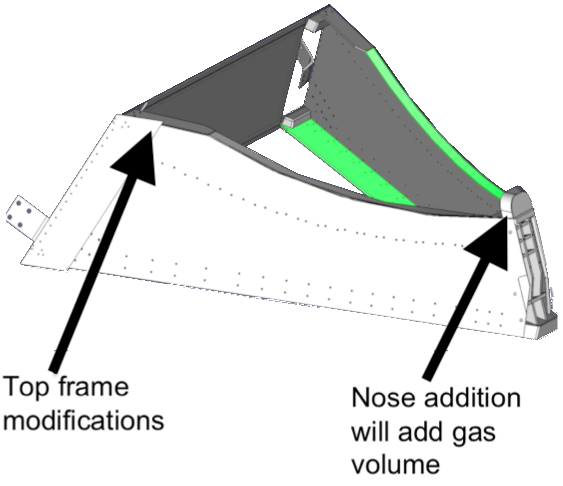
\includegraphics[width=1.0\columnwidth, height=0.75\columnwidth]{img/boxCut.png}
	\caption{The refurbished LTCC frame. Originally the frame walls had a 5m radius sphere centered on the target profile.
            The side-walls had to be cut near the top part of the box and the three mirror sets involved had to be relocated.
				At the bottom of the box, a stainless steel nose window support was added to the original detector to increase the gas volume.}
	\label{fig:boxCut}
\end{figure}


\subsection{Nose addition and window inflation}

In the original design the upstream window followed the spherical curvature of the frame sidewalls. In the new design, the window is left to inflate
to enlarge the gas volume in order to increase the number of Cherenkov photons. In addition, a ``nose'' support (see \F{boxCut}) has been engineered to
increase the gas volume.
The nose dimensions have been optimized to provide the best support while at the same time maximize the gas volume increase. The gas volume increase
of the final configuration is shown in \F{noseVolume}.


\begin{figure}
	\centering
	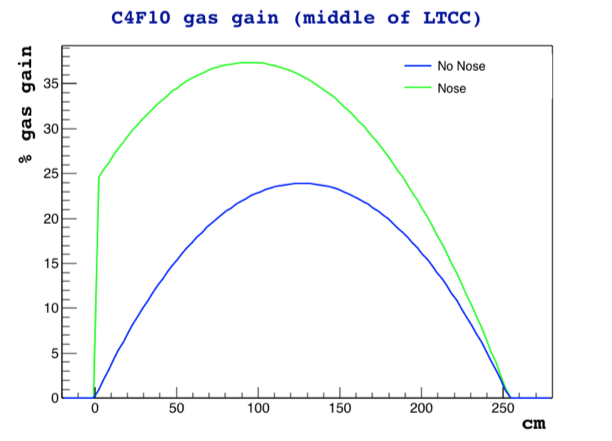
\includegraphics[width=0.98\columnwidth, height=0.7\columnwidth]{img/noseVolume.png}
	\caption{The gas volume percentage gains with and without the nose addition compared to the old CLAS configuration as a function of
            distance from the nose in cm. Blue: the percentage increase due to the window inflation compared to the original flat design.
            Green: the additional percentage increase due to the nose addition.}
	\label{fig:noseVolume}
\end{figure}


\subsection{Back-wall and connectors}

Both the high voltage and the signals connector that link the PMTs inside the hermetical box and the electronics were not
hermetical during CLAS operations and epoxy was used to minimize the leaks from these connectors.
As part of the back-wall refurbishment, the patch panel was rebuilt and hermetical connectors were used.

The new back wall design is shown in \F{backWall}. The wall is supported by stainless steel bars that enclose a panel made of foam enclosed by
thin aluminum sheets to minimize the radiation length.
The new patch panels provide 3 connectors for each PMT: one for high voltage and two for an identical signal coming from the modified PMT base.
One signal is digitized through flash ADC and the other one through a discriminator TDC.

\begin{figure}
	\centering
	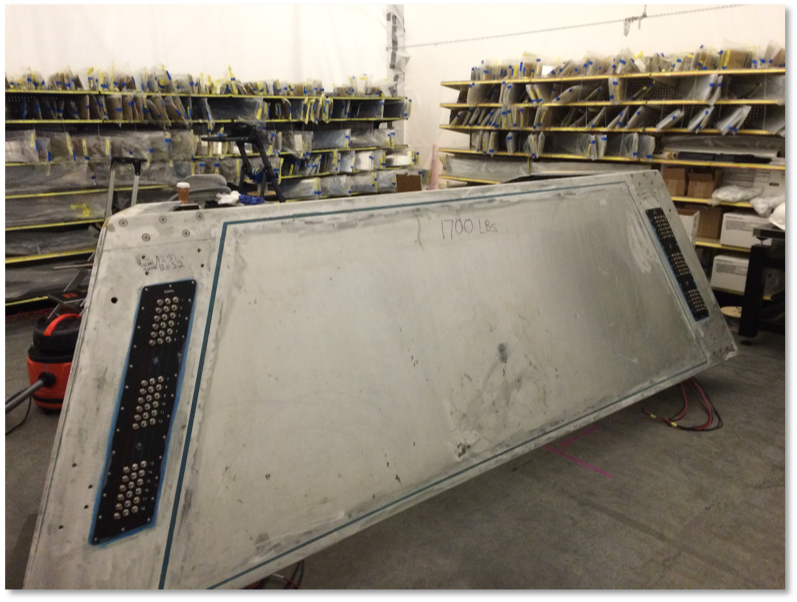
\includegraphics[width=0.95\columnwidth,keepaspectratio]{img/backWall.png}
	\caption{Top view of the back-wall of the LTCC. A stainless steel bar encapsulate a sandwich wall of aluminum and foam. On the left and right side
            of the frame new patch panels allow for 3 hermetical BNC RG58 connectors (1 HV, 2 signals) from each PMT. }
	\label{fig:backWall}
\end{figure}


\subsection{Mirror support spine}

When opened for refurbishment, the mirror support spine of all six LTCC sectors were found to be broken. The spine was an aluminum honeycomb designed to prevent
the mirrors from breaking under their own weight. It was attached to the box nose and the back-wall. The spine was rigid and broke due to small
(of the order of 0.5 cm) deformations of the box when it was transported and/or installed.
A new carbon fiber spine, see \F{spine}, was designed capable of floating up to 1 cm, effectively compensating for the non rigid movements of the box.
The mirrors are linked to the spine through stainless steel cables 0.127 mm thick. The cables were anchored with stainless steel springs with tension varying from 0.5 to 1 Kg.
The spine was tested by mounting a laser on the box. Its laser line was focused through the elliptical and hyperbolic mirrors to a target in the middle of the covered face of a PMT.
In order to verify that the detector transportation and/or installation would not break the spine nor affect the mirror alignment, the box was lifted,
rotated back and forth by 90 degrees, and subjected to small vibrations, see \F{spineTest}. The focused spot on the PMT did not change with any of these movement and the spine
compensated for the walls deformations.

\begin{figure}
	\centering
	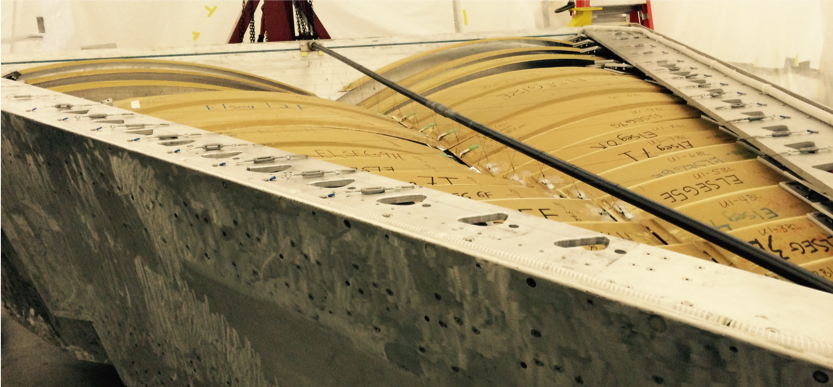
\includegraphics[width=1.0\columnwidth,keepaspectratio]{img/spine.png}
	\caption{The LTCC mirror support spine. The carbon fiber tube (in black) is allowed to float up to 1cm to compensate for possible box deformation during the detector
            transportation and installation. The mirrors re linked to the spine through stainless steel cables 0.127 mm thick and tensioned through springs.}
	\label{fig:spine}
\end{figure}


\begin{figure}
	\centering
	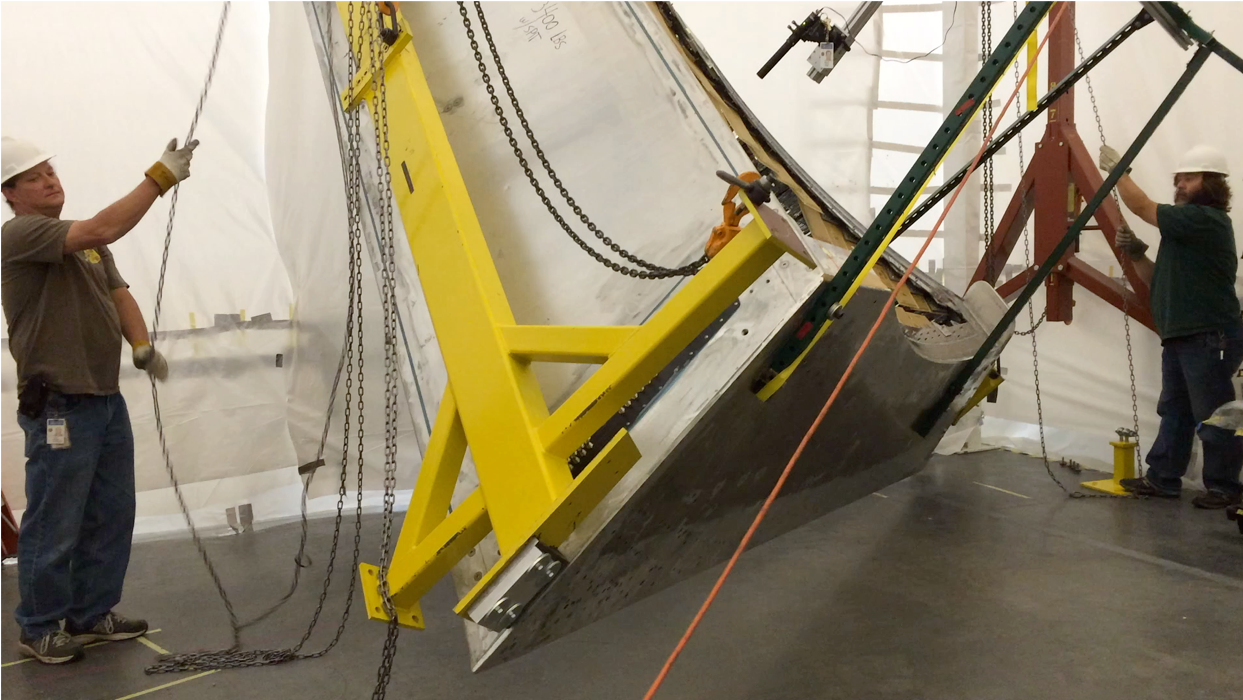
\includegraphics[width=1.0\columnwidth,keepaspectratio]{img/spineTest.png}
	\caption{Spine tests: a laser was mounted on a structure attached to one LTCC sector, pointing a laser line that was focused by the mirrors to a
            target on the face of one PMT. The focused laser spot never changed during the box movements and rotations.}
	\label{fig:spineTest}
\end{figure}





